\section{Flow: overview}
\label{sec:flow-overview}

% Flow: application components description
In this section, we first describe an overview of the Flow application, and then the design goal of this application.

Flow is a prototype of a multi-user ``exploration game'', in which participants navigate and interact with a virtual world rendered in a game engine using a combination of inputs: 
\begin{enumerate}
\item \textit{Indoor positioning}: participants' positions in physical space, detected by indoor positioning (person tracking), modify the virtual landscape;
\item \textit{Wearable sensing}: participants directly control orientation of the environment's virtual camera using gyroscopes connected to  microcontrollers, which can be worn or carried; 
\item \textit{Mobile phone interface}: participants interact with the virtual environment through controls on their smartphone, for example to share social media images in the virtual environment.
\end{enumerate}
In addition to various types of IoT devices and the game engine, the system on which Flow is built also includes an \textit{authentication server} (AS) that performs local trust management.
The AS can be implemented as an app on the owner's smartphone, or a service daemon on a dedicated control hub (e.g., the home router).

\begin{figure}[!t]
\centering
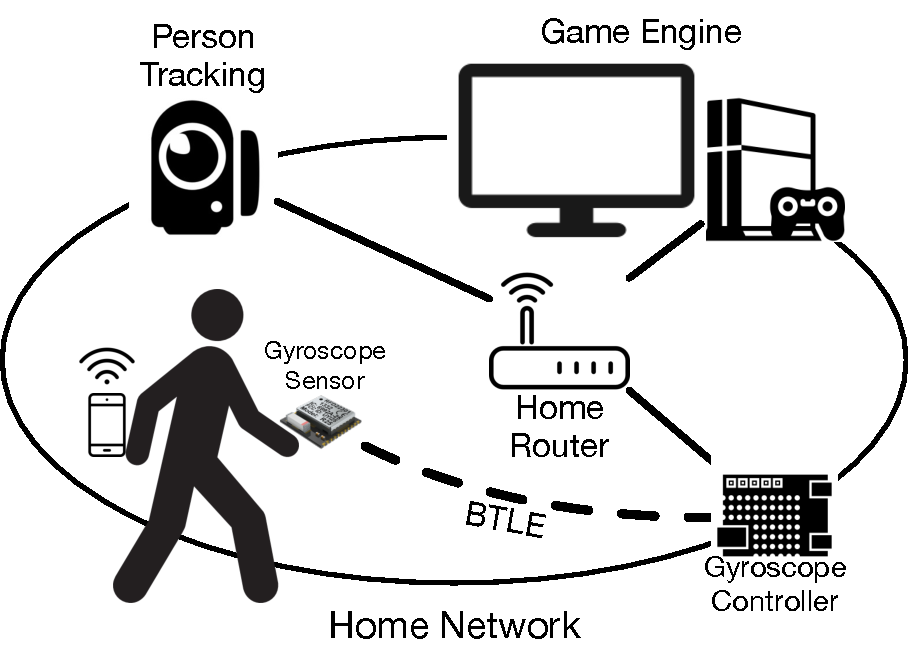
\includegraphics[width=0.9\columnwidth]{flow-home-deployment.pdf}
\caption{Typical deployment of the Flow home entertainment experience.}
\label{fig:flow-deployment}
\end{figure}

Figure~\ref{fig:flow-deployment} shows a typical deployment scenario of Flow in a home network.  NDN interconnectivity between different components is supported over Ethernet and Wi-Fi, through the home Wi-Fi router in a hub-and-spoke topology. 

Sensor devices with limited networking capability (e.g., the gyroscope in Fig.~\ref{fig:flow-deployment}) may be bridged via a helper device.
We assume all devices can reach each other over NDN, which is trivial in a hub-and-spoke topology.\footnote{A routing protocol may be required if a sensor mesh topology is deployed inside the home network.}

% goal: local communication and security
% Flow adopts a cloudless architecture, and uses the NDN protocol stack to connect hardware with varying capabilities, as well as secure a diverse range of sensing data.
The design of Flow application focuses on cloudless communication (while local reachability is a minor concern) and security (signing and verification).

While analyzing the requirement of Flow, we re-examined the building blocks described in Section IV of cite:iotdi-2016 paper, and found them helpful for the implementation of Flow application, as well as traditional home automation systems and many other IoT subdomains. 
Thus we designed NDN-IoT framework to provide the following abstractions
naming: easily support multiple levels of names
bootstrap: AS component and device onboarding
discovery: 
can support various types of devices that Flow application requires

